%!TEX TS-program = xelatex
\documentclass[xetex,10pt,aspectratio=43]{beamer} 
%设置为 Beamer 文档类型,设置字体为 10pt,长宽比为16:9,数学字体为 serif 风格
\batchmode

\usefonttheme{professionalfonts}
\usetheme{Berlin} %主题
\usecolortheme{sustech} %主题颜色

\usepackage[UTF8]{ctex}
\usepackage{unicode-math}
\usepackage{graphicx}
\usepackage{animate}
\usepackage{tikz}
\usepackage{hyperref}

%导入一些用到的宏包
\usepackage{amsmath,bm,amssymb,enumerate,epsfig,bbm,calc,color,ifthen,capt-of,multimedia}
\usepackage[ruled,linesnumbered]{algorithm2e}

\usepackage{fancybox}
\usepackage{xcolor}
\usepackage{times}
\usepackage{listings}

\usepackage{booktabs}
\usepackage{colortbl}

\newcommand{\Console}{Console}
\lstset{ %
	backgroundcolor=\color{white},   % choose the background color
	basicstyle=\footnotesize\rmfamily,     % size of fonts used for the code
	columns=fullflexible,
	breaklines=true,                 % automatic line breaking only at whitespace
	captionpos=b,                    % sets the caption-position to bottom
	tabsize=4,
	commentstyle=\color{mygreen},    % comment style
	escapeinside={\%*}{*)},          % if you want to add LaTeX within your code
	keywordstyle=\color{blue},       % keyword style
	stringstyle=\color{mymauve}\ttfamily,     % string literal style
	numbers=left, 
	%	frame=single,
	rulesepcolor=\color{red!20!green!20!blue!20},
	% identifierstyle=\color{red},
	language=c
}

\setmathfont{XITS Math}

\definecolor{mygreen}{rgb}{0,0.6,0}
\definecolor{mymauve}{rgb}{0.58,0,0.82}
\definecolor{mygray}{gray}{.9}
\definecolor{mypink}{rgb}{.99,.91,.95}
\definecolor{mycyan}{cmyk}{.3,0,0,0}

%题目,作者,学校,日期
\title{离散数学基础}
\subtitle{\fontsize{9pt}{14pt}\textbf{集合等式}}
\author{中山大学MOOC课程组}
\institute{\fontsize{8pt}{14pt}中山大学计算机学院}
\date{\today}

%学校Logo
%\pgfdeclareimage[height=0.5cm]{sustech-logo}{sustech-logo.pdf}
%\logo{\pgfuseimage{sustech-logo}\hspace*{0.3cm}}

\AtBeginSection[]
{
	\begin{frame}<beamer>
		\frametitle{\textbf{目录}}
		\tableofcontents[currentsection]
	\end{frame}
}
\beamerdefaultoverlayspecification{<+->}

%图片
\graphicspath{{img/}}

%幂集
\newcommand{\powerset}{\raisebox{.15\baselineskip}{\ensuremath{\wp}}}
% -----------------------------------------------------------------------------
\begin{document}
	% -----------------------------------------------------------------------------
	
	\frame{\titlepage}
	
	\section[目录]{}   %目录
	\begin{frame}{目录}
		\tableofcontents
	\end{frame}

	\section{基本知识回顾}
	
	\subsection{基于定义证明集合等式}
	
	\begin{frame}{基于定义证明集合等式}
		
		根据集合相等的定义,通过考察一个集合的元素是否相互属于另一个集合而证明集合等式。
		
		\vspace{0.5cm}
		
		证明$A=B$的最直接模式:
		
		对任意$x$,$x\in A$ 当且仅当 $\dots$
		
		\qquad\qquad\qquad\qquad\qquad$\vdots$
		
		\qquad\qquad\qquad\qquad 当且仅当$x\in B$	
		
		\vspace{0.5cm}
		
		也可以使用定理$A=B\equiv A\subseteq B\wedge B\subseteq A$
		
	\end{frame}


	\begin{frame}{证明对任意集合$A$,$\bigcup \powerset(A)=A$}
	
	使用定理$A=B\equiv A\subseteq B\wedge B\subseteq A$
	
	\begin{block}<1>{$\bigcup \powerset(A)\subseteq A$}
		
		对任意$x$,若$x\in \bigcup\powerset(A)$,则存在$S\in \powerset(A)$使得$x\in S$,$S\subseteq A$,故有$x\in A$
		
	\end{block}
	
	\begin{block}<1>{$A\subseteq\bigcup \powerset(A)$}
		
		对任意$x$,若$x\in A$,因为$A\in \powerset(A)$,故$x\in \bigcup\powerset(A)$
		
	\end{block}
	
	\end{frame}

	\begin{frame}{对称差}
	
	集合$A$和$B$的对称差记为$A\oplus B$。\textcolor{red}{对称差的相关证明较难,可以使用成员关系表证明,文氏图不能作为严格的证明方法。}
	
	$$A\oplus B=\{x|(x\in A\wedge x\notin B)\vee(x\notin A\wedge x\in B)\}$$
	
	\begin{columns}
		
	\begin{column}<1>{0.5\textwidth}
			
	\begin{figure}
				
	\centering
	
	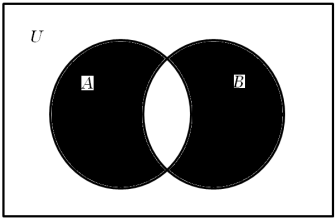
\includegraphics[scale=0.4]{4.png}
	
	\caption{集合$A\oplus B$的文氏图}
		
	\end{figure}
			
	\end{column}
		
	\begin{column}<1>{0.5\textwidth}
		
	\begin{table}
		
	\centering
	
	\begin{tabular}{|c|c|c|}
		\hline
		$A$ & $B$ & $A\oplus B$\\
		\hline
		0 & 0 & 0\\
		\hline
		0 & 1 & 1\\
		\hline
		1 & 0 & 1\\
		\hline
		1 & 1 & 0\\
		\hline
	\end{tabular}
	
	\caption{集合$A\oplus B$的成员关系表}
		
	\end{table}
		
	\end{column}
		
	\end{columns}
	
	\end{frame}

	\begin{frame}{证明对称差运算的结合性}
		
		\centering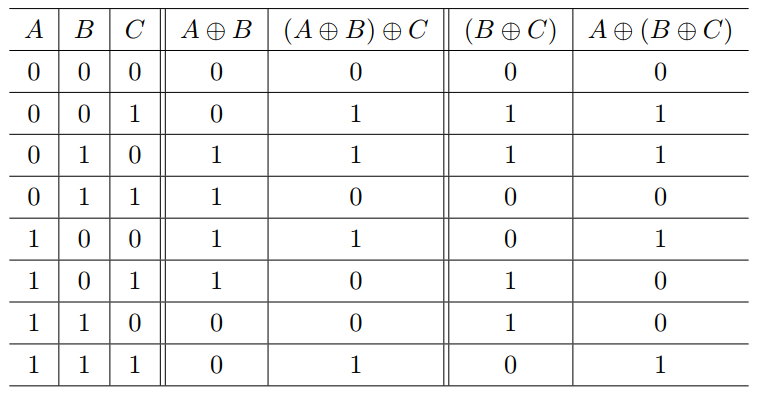
\includegraphics[scale=0.5]{1.png}
		
		\textcolor{red}{对称差的相关证明较难,可以使用成员关系表证明。}	
		
	\end{frame}
	
	\subsection{集合等式演算}
	
	\begin{frame}{集合等式演算}
		
	\begin{figure}
		
		\centering
		
		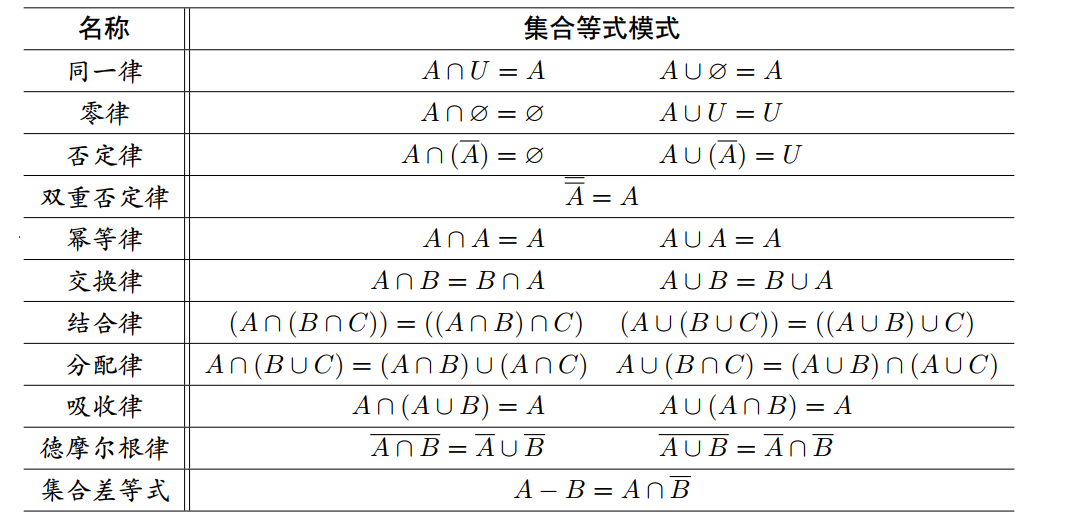
\includegraphics[scale=0.4]{5.png}
		
		\caption{基本的集合等值模式}
		
	\end{figure}
		
	\end{frame}

	\begin{frame}{证明集合差的德摩尔根率}
	
	\begin{block}<1>{$A-(B\cap C)=(A-B)\cup(A-C)$}
	
	$A-(B\cap C)=A\cap\overline{(B\cap C)}$
	
	$A-(B\cap C)=A\cap(\overline{B}\cup\overline{C})$
	
	$A-(B\cap C)=(A\cap\overline{B})\cup(A\cap\overline{C})$

	$A-(B\cap C)=(A-B)\cup(A-C)$
	
	\end{block}
	
	\begin{block}<1>{$A-(B\cup C)=(A-B)\cap(A-C)$}
	
	$A-(B\cup C)=A\cap\overline{(B\cup C)}$
	
	$A-(B\cup C)=A\cap(\overline{B}\cap\overline{C})$
	
	$A-(B\cup C)=(A\cap\overline{B})\cap(A\cap\overline{C})$
	
	$A-(B\cup C)=(A-B)\cap(A-C)$
		
	\end{block}

	\end{frame}
	
	\subsection{子集关系与集合等式}
	
	\begin{frame}{子集关系与集合等式}
		
	根据我们在前两节课学习的定理来进行证明
		
	\end{frame}

	\begin{frame}{对任意集合$A$和$B$,$A\subseteq B$当且仅当$A\cap B=A$当且仅当$A\cup B=B$}
	
	易得$A\cap B\subseteq A$,当$A\subseteq B$时,$\forall x\in A$,$x\in B$,故$x\in A\wedge B$,故$A\subseteq A\cap B$
	
	易得$A\cap B\subseteq B$,当$A\cap B=A$时,$A\subseteq B$
	
	易得$B\subseteq A\cup B$,当$A\subseteq B$时,$A\cup B\subseteq B$
	
	易得$A\subseteq A\cup B$,当$A\cup B=B$时,$A\subseteq A\cup B=B$
	
	\end{frame}

	\begin{frame}{对任意集合$A$,$B$,$C$,$D$,若$A\subseteq C$且$B\subseteq D$,则$A\cap B\subseteq C\cap D$,$A\cup B\subseteq C\cup D$}
		
	因为$A\cap B\subseteq A$,$A\subseteq C$,故$A\cap B\subseteq C$,因为$A\cap B\subseteq B$,$B\subseteq D$,故$A\cap B\subseteq D$,故$A\cap B\subseteq C\cap D$
	
	因为$A\subseteq C$,$C\subseteq C\cup D$,故$A\subseteq C\cup D$,故$A\subseteq C\cup D$,因为$B\subseteq D$,$D\subseteq C\cup D$,故$B\subseteq C\cup D$,故$B\subseteq C\cup D$,故$A\cup B\subseteq C\cup D$
	
	\vspace{0.5cm}
		
	\textcolor{red}{集合交,并,幂运算保持子集关系不变}
	
	\end{frame}

	\begin{frame}{设$A\subseteq B$且$A\cap C=\varnothing$,则$A\subseteq B-C$}
		
	$B-C=B\cap\overline{C}$
	
	$A\cap C=\varnothing\rightarrow \overline{A}\cup\overline{C}=U\rightarrow A\cap\overline{C}=A\subseteq\overline{C}$
	
	\end{frame}

	\begin{frame}{$A$,$B$,$C$是集合,证明$A\cup C\subseteq B\cup C$当且仅当$A-C\subseteq B-C$}
		
	当$A\cup C\subseteq B\cup C$,$\overline{C}\cap(A\cup C)\subseteq \overline{C}\cap(B\cup C)\rightarrow A\cap\overline{C}\subseteq B\cap\overline{C}$
	
	当$A-C\subseteq B-C$,$A\cap\overline{C}\subseteq B\cap\overline{C}\subseteq B\rightarrow C\cup(A\cap\overline{C})\subseteq C\cup B\rightarrow A\cup C\subseteq B\cup C$
	
	\end{frame}

	\begin{frame}{证明$\overline{A\cup B}=\overline{A}\cap\overline{B}$}
	
	利用$A=B\equiv A\subseteq B\wedge B\subseteq A$
	
	\begin{block}<1>{$\overline{A\cup B}\subseteq\overline{A}\cap\overline{B}$}

	$A\subseteq A\cup B\rightarrow\overline{A\cup B}\rightarrow\overline{A}$
	
	$B\subseteq A\cup B\rightarrow\overline{A\cup B}\rightarrow\overline{B}$
	
	$\overline{A\cup B}\rightarrow\overline{A}\cap\overline{B}$
		
	\end{block}

	\begin{block}<1>{$\overline{A}\cap\overline{B}\subseteq\overline{A\cup B}$}
	
	$\overline{A}\cap\overline{B}\subseteq\overline{A}\rightarrow A\subseteq\overline{\overline{A}\cap\overline{B}}$
	
	$\overline{A}\cap\overline{B}\subseteq\overline{B}\rightarrow B\subseteq\overline{\overline{A}\cap\overline{B}}$
	
	$A\cup B\subseteq\overline{\overline{A}\cap\overline{B}}\rightarrow\overline{A}\cap\overline{B}\subseteq\overline{A\cup B}$
		
	\end{block}
	
	\end{frame}

	\begin{frame}{$\powerset(A)\cup\powerset(B)\subseteq\powerset(A\cup B)$}
	
	由上节课的定理可知,幂集运算保持子集关系,$A\subseteq B\rightarrow\powerset(A)\subseteq\powerset(B)$
	
	$A\subseteq A\cup B\rightarrow\powerset(A)\subseteq\powerset(A\cup B)$
	
	$B\subseteq A\cup B\rightarrow\powerset(B)\subseteq\powerset(A\cup B)$
	
	$\powerset(A)\cup\powerset(B)\subseteq\powerset(A\cup B)$
	
	\end{frame}

	\section{习题讲解}
	
	\begin{frame}{若$A\cap B=A\cap C$且$A\cup B=A\cup C$,则$B=C$}
	
	利用$A=B\equiv A\subseteq B\wedge B\subseteq A$	
	
	\begin{block}<1>{$B\subseteq C$}
	
	对任意$x\in B$,若$x\in A$,有$x\in A\cap B=A\cap C\subseteq C$,故$x\in C$
	
	若$x\notin A$,$x\in B\subseteq A\cup B=A\cup C$,$x\in C$
		
	\end{block}

	\begin{block}<1>{$C\subseteq B$}
	
	对任意$x\in C$,若$x\in A$,有$x\in A\cap C=A\cap B\subseteq B$,故$x\in B$
	
	若$x\notin A$,$x\in C\subseteq A\cup C=A\cup B$,$x\in B$
	
	\end{block}
		
	\end{frame}

	\begin{frame}{证明$A\cap(B\oplus C)=(A\cap B)\oplus(A\cap C)$}
			
	\begin{table}
		
	\centering
	
	\begin{tabular}{|c|c|c|c|c|c|c|c|}
		\hline
		$A$ & $B$ & $C$ & $B\oplus C$ & $A\cap B$ & $A\cap C$ & $A\cap(B\oplus C)$ & $(A\cap B)\oplus(A\cap C)$\\
		\hline
		0 & 0 & 0 & 0 & 0 & 0 & 0 & 0\\
		\hline
		0 & 0 & 1 & 1 & 0 & 0 & 0 & 0\\
		\hline
		0 & 1 & 0 & 1 & 0 & 0 & 0 & 0\\
		\hline
	 	0 & 1 & 1 & 0 & 0 & 0 & 0 & 0\\
		\hline
		1 & 0 & 0 & 0 & 0 & 0 & 0 & 0\\
		\hline
		1 & 0 & 1 & 1 & 0 & 1 & 1 & 1\\
		\hline
		1 & 1 & 0 & 1 & 1 & 0 & 1 & 1\\
		\hline
		1 & 1 & 1 & 0 & 1 & 1 & 1 & 1\\
		\hline
	\end{tabular}
		
	\end{table}
	
	\textcolor{red}{对称差的相关证明较难,可以使用成员关系表证明。}
	
	\end{frame}
	
	\begin{frame}{若$(A\cap B)\cup C=A\cap(B\cup C)$当且仅当$C\subseteq A$}
	
	\begin{block}<1>{必然性}
		
	$C\subseteq (A\cap B)\cup C=A\cap(B\cup C)\subseteq A$
		
	\end{block}

	\begin{block}<1>{充分性}
	
	\begin{itemize}
		
		\item<1> $(A\cap B)\cup C\subseteq A\cap(B\cup C)$

		$A\cap B\subseteq A$,$C\subseteq A$,故$(A\cap B)\cup C\subseteq A$
		
		$(A\cap B)\cup C=(A\cup C)\cap(B\cup C)\subseteq(B\cap C)$
				
		\item<1> $A\cap(B\cup C)\subseteq (A\cap B)\cup C$
		
		$A\cap(B\cup C)=(A\cap B)\cup(A\cap C)$
		
		$A\cap B\subseteq(A\cap B)\cup C$
		
		$A\cap C\subseteq(A\cap B)\cup C$
		
	\end{itemize}
	
	\end{block}
		
	\end{frame}

	\begin{frame}{若$\powerset(A)\cup\powerset(B)=\powerset(A\cup B)$,则$A\subseteq B$或$B\subseteq A$}
	
	反证法
	
	若存在$x_1\in A-B$,$x_2\in B-A$,${x_1,x_2}\in \powerset(A\cup B)=\powerset(A)\cup\powerset(B)$
	
	${x_1,x_2}\notin \powerset(A)$,${x_1,x_2}\notin \powerset(B)$,矛盾
		
	\end{frame}

	\section{总结}
	
	\begin{frame}{总结}
	
	这一节的主要内容有:
	
	\begin{itemize}
		
		\item<1> 证明集合等式
		
		\item<1> 证明子集关系
		
	\end{itemize}

	
	\vspace{0.5cm}

	用到的方法有:
	
	一二节的定义,等值模式,定理($A=B\equiv A\subseteq B\wedge B\subseteq A$),成员关系表...
		
	\vspace{0.5cm}
	
	\textcolor{red}{定理比较多,不需要死记硬背,重点把一二节的定义掌握好就可以了,包括集合关系的定义,集合运算的定义。}
	
	\end{frame}
	
	\begin{frame}{Thank you}
		\begin{center}
			\begin{minipage}{\textwidth}
				\setbeamercolor{mybox}{fg=white, bg=black!50!blue}
				\begin{beamercolorbox}[wd=0.70\textwidth, rounded=true, shadow=true]{mybox}
					\LARGE \centering Thank you for listening!  %结束语
				\end{beamercolorbox}
			\end{minipage}
		\end{center}
	\end{frame}
	
	
	% -----------------------------------------------------------------------------
\end{document}
%文档结束
